% You should title the file with a .tex extension (hw1.tex, for example)
\documentclass[a4paper, 11pt]{article}

\usepackage{amsmath}
\usepackage{amssymb}
\usepackage{fancyhdr}
\usepackage{graphicx}

\usepackage[margin=1in]{geometry}

\newcommand{\question}[2] {\vspace{.25in} \hrule\vspace{0.5em}
\noindent{\bf #1: #2} \vspace{0.5em}
\hrule \vspace{.10in}}
\renewcommand{\part}[1] {\vspace{.10in} {\bf (#1)}}

\newcommand{\myname}{Natthakan Euaumpon}
\newcommand{\myemail}{natthakaneuaumpon@gmail.com}
\newcommand{\myhwnum}{6}

\setlength{\parindent}{0pt}
\setlength{\parskip}{5pt plus 1pt}
 
\pagestyle{fancyplain}
\lhead{\fancyplain{}{\textbf{HW\myhwnum}}}      % Note the different brackets!
\rhead{\fancyplain{}{\myname\\ \myemail}}
\chead{\fancyplain{}{ICCS310 }}

\begin{document}

\medskip                        % Skip a "medium" amount of space
                                % (latex determines what medium is)
                                % Also try: \bigskip, \littleskip

\thispagestyle{plain}
\begin{center}                  % Center the following lines
{\Large ICCS310: Assignment \myhwnum} \\
\myname \\
\myemail \\
March 2021 \\
\end{center}

\question{1}{The Meaning of Things}
\part{1}{Give a definition of the class NP}\\
Complexity class used to classify problems. It is a set of problem that can be check if true within polynomial time. 

\part{2}{Explain how one can prove that a problem belongs to the class NP}\\
Show that the problems have certificate and verifier and that the problem can be check in polynomial time.

\part{3}{What is NP-complete?}\\
The complexity class of decision problems in NP and no other NP problem is harder.

\part{4}{Describe a startegy for showing that a problem is NP-complete}\\
Show that the problem is in NP and that the problem can be reduces to alredy known np-complete problem (NP-hard).

\question{2}{Closure of NP}
\part{1}{$A \cap B$ must be in NP}\\
Let $A = L_1$ and $B = L_2$. For $i$ = 1,2 let $V_i(x,c)$ be an algorithm such that x is a string, c is a possible certificate and this algorithm will verify whether c is a certificate for $x \in L_i$. If certificates c verifies $x \in L_i$ then $V_i(x,c) = 1$. Else $V_i(x,c) = 0$. Since we know that both $L_1$ and $L_2$ are in NP. Then we know that algorithm $V_i(x,c)$ terminates in polynomial time which is $O(|x^d|)$. Where d is a constant. Let construct another verifier called $V_3$ which verify $L_1 \cap L_2$. Let $L_1 \cap L_2 = L_3$. Then $V_3 = V_1 \cap V_2$. This clearly indicate that $x \in L_3$ if and only if there is a certificate $c$ suchthat $V_3(x,c) = 1$. Then this verifier will run in $O(2(|x|^d))$ which is in polynomial time. Therefore $L_3$ is also in NP. So, $A \cap B$ is in NP.

\part{2}{$A \cup B$ must be in NP}\\
Let $A = L_1$ and $B = L_2$ For $i$ = 1,2 let $V_i(x,c)$ be an algorithm such that $x$ is a string, $c$ is a possible certificate and this algorithm will verify whether $c$ is a certificate for $x \in L_i$. If certificates c verifies $x \in L_i$ then $V_i(x,c) = 1$. Else $V_i(x,c) = 0$. Since we know that both $L_1$ and $L_2$ are in NP. Then we know that algorithm $V_i(x,c)$ terminates in polynomial time which is $O(|x^d|)$. Where d is a constant. Let construct another verifier called $V_3$ which verify $L_1 \cup L_2$. Let $L_1 \cup L_2 = L_3$. Then $V_3 = V_1 \cup V_2$. This clearly indicate that $x \in L_3$ if and only if there is a certificate $c$ suchthat $V_3(x,c) = 1$. Then this verifier will run in $O(2(|x|^d))$ which is in polynomial time. Therefore $L_3$ is also in NP. So, $A \cup B$ is in NP.

\question{3}{This is NP}
certificate = colour assignment of each vertex.\\
verifier = run throgh and check if for each edge $(u,v)$, the colour of $u$ is different from that of $v$.

\question{4}{NP-Complete}
\part{1}{Prove that HAM-PATH is NP-complete}
From class we know that 3-SAT is in NP-Complete.\\
$HAMPATH = (G,s,t)$ where G is a directed graph with a Hamiltonian path from s to t.\\ 
For a given k clauses:\\
$\phi = (a_1 \lor b_1 \lor c_1) \land (a_2 \lor b_2 \lor c_2) \land ... \land (a_k \lor b_k \lor c_k)$\\
Let $(a_1 \lor b_1 \lor c_1) = c_1$, $(a_2 \lor b_2 \lor c_2) = c_2$ ... $((a_k \lor b_k \lor c_k)) = c_k$ and $a_i,b_i,c_i$ are literals $x$ or $\overline{x}$, $i=k$. Let $x_1 ... x_l$ be the $l$ variable of $\phi$. Let construct graph G where each $x_i$ is represented with a diamond-shaped structure such that each diamond contain a horizontal row of nodes where it is connected by edges running in both direction.The horizontal row contains $2k$ nodes,  $k-1$ extra node in between every 2 node from the clause and 2 nodes on the top and bottom to form a diamond shape. So the total number of node is $2k + (k-1) + 2 = 3k+1$ nodes. If $x_i$ appears in the clause then we add two edges from the pair in the ith diamond to the clause node. \\
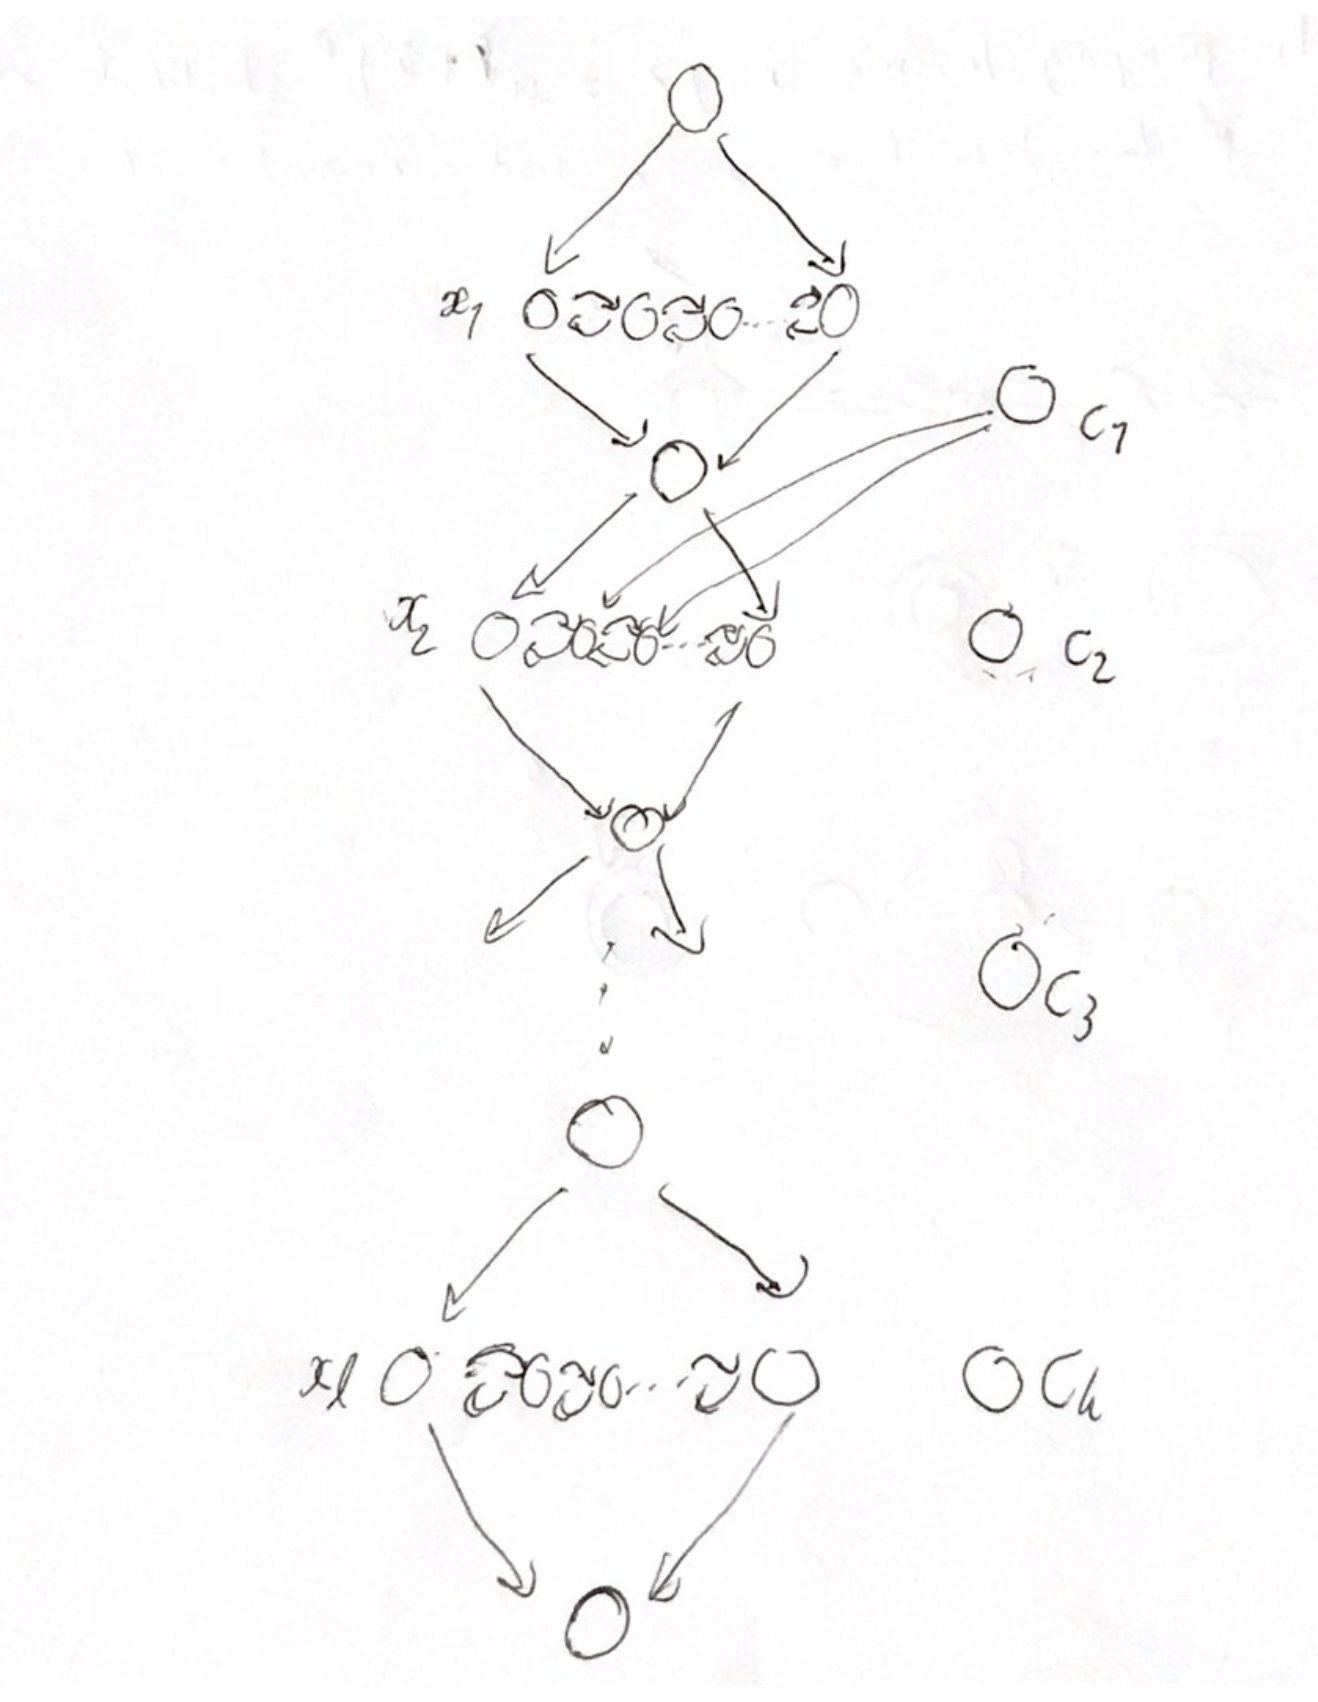
\includegraphics[width=\textwidth]{Q4-1.png}\\
Suppose that $\phi$ is satisfiable, then a Hamiltonian path exists from s to t. To show this (Follow the blue arrow):\\
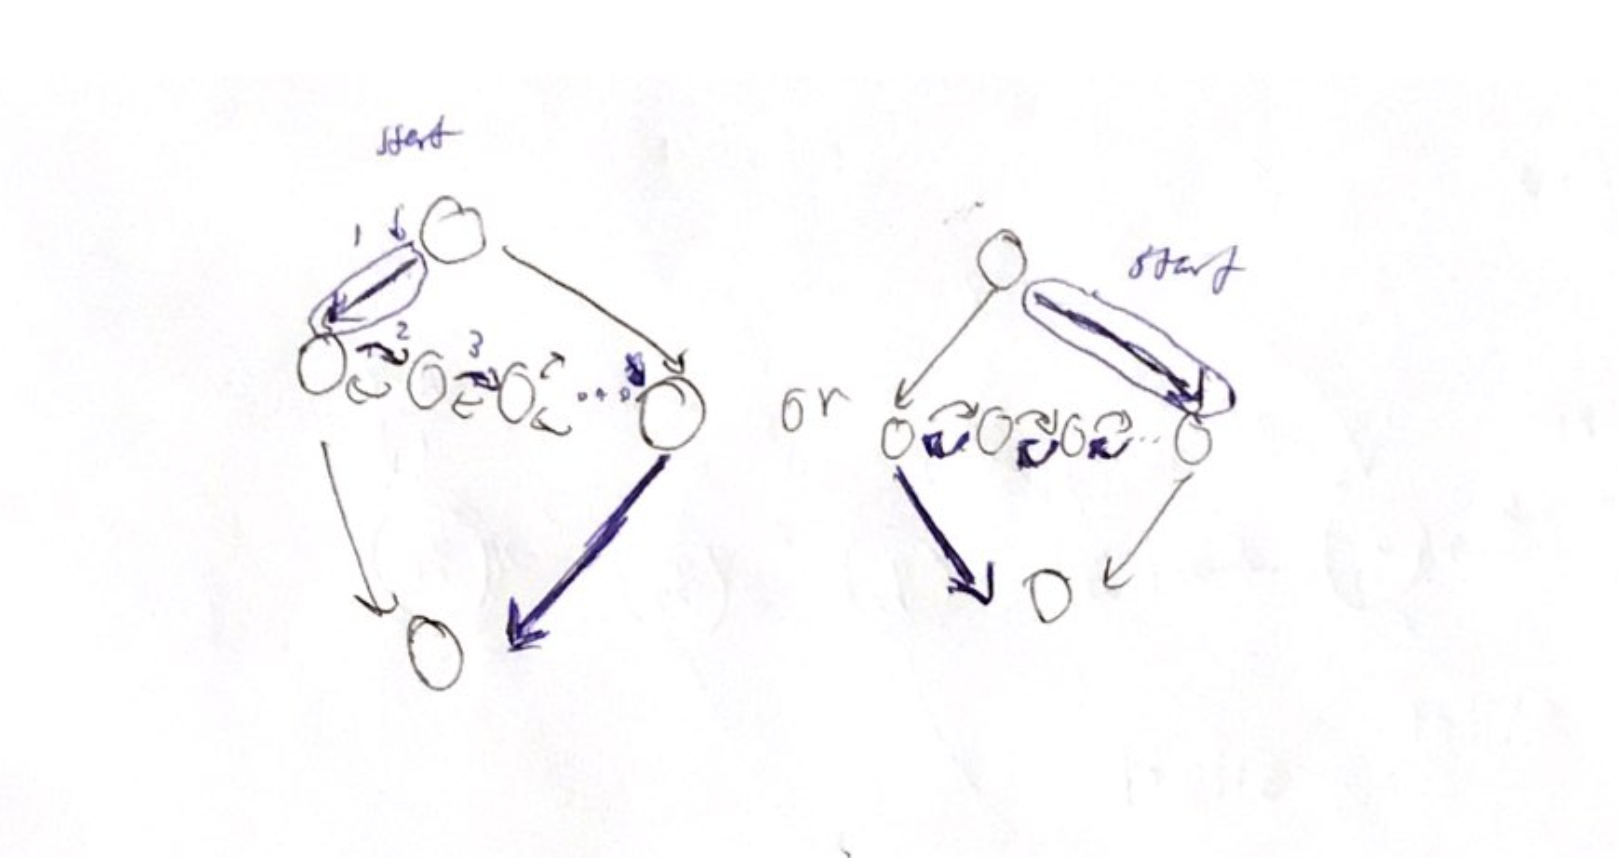
\includegraphics[width=\textwidth]{Q4-2.png}\\
To cover the clause nodes $c_j$ then we can make a detour as follow:\\
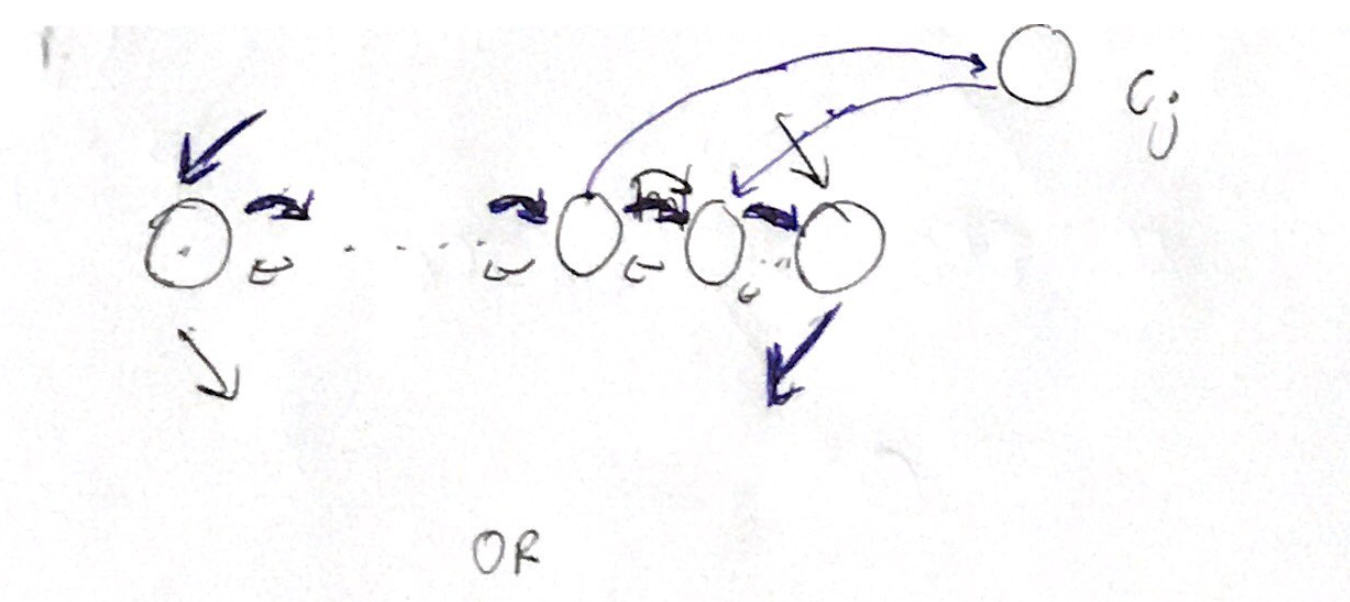
\includegraphics[width=\textwidth]{Q4-4.png}\\
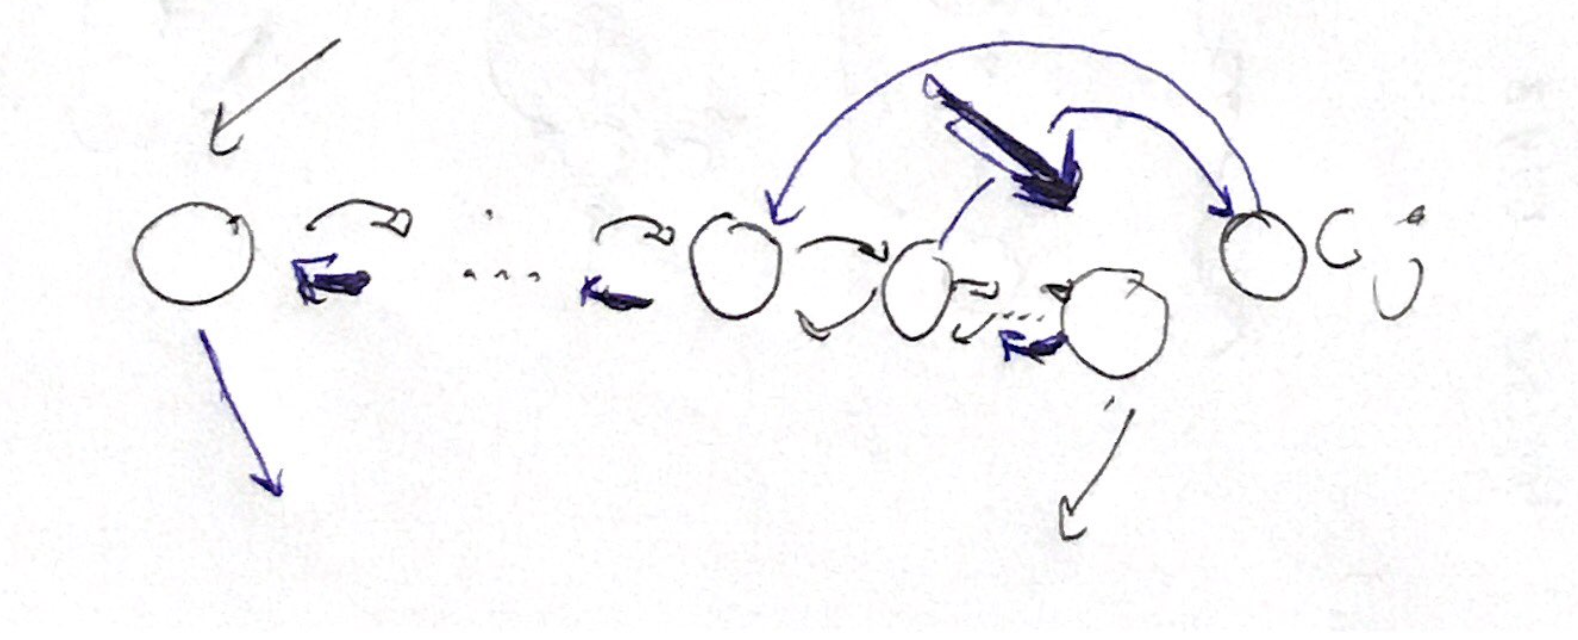
\includegraphics[width=\textwidth]{Q4-6.png}\\
This case cannot happend:\\
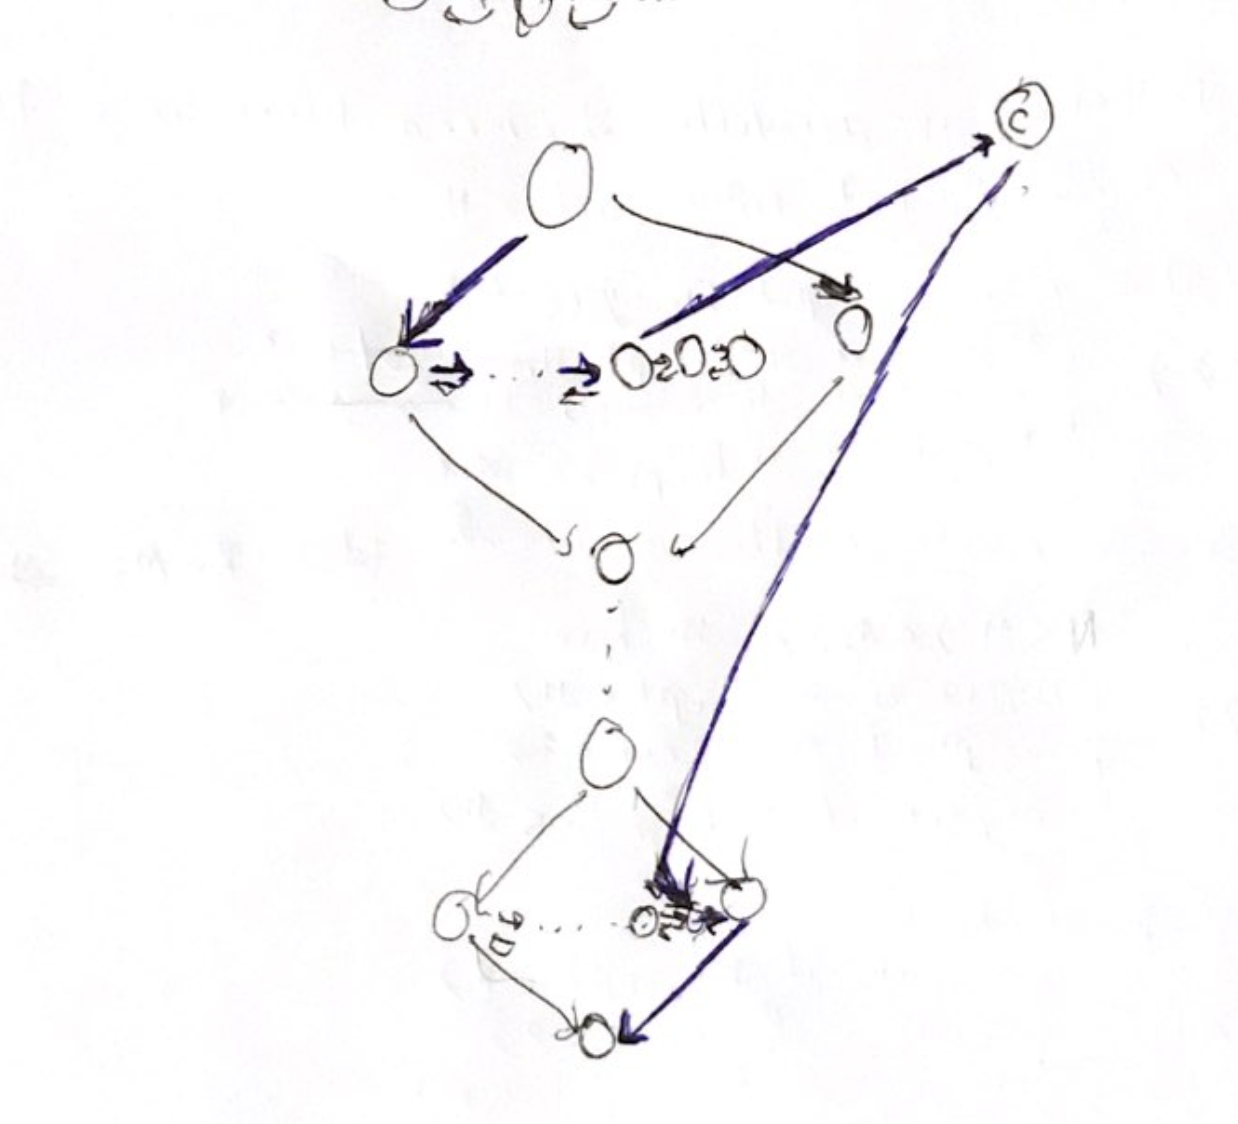
\includegraphics[width=\textwidth]{Q4-3.png}\\
This prove that this reduction works. Hence $3-SAT \leq_m HAM-PATH$.

\part{2}{Prove that UNDIRECTED-HAM-PATH is NP-complete}\\
We just prove that HAM-PATH is NP-complete.\\
$UNDIRECTEDHAMPATH = (G,s,t)$ where G is a directed graph with a Hamiltonian path from s to t.\\ 
Let $s$ in $G$ map to $s^{out}$ in $G^{'}$ and $t$ in $G$ map to $t^{in}$ in $G^{'}$. Other node $u_i$ in $G$ become edges incident on $u_i^{in}, u_i^{middle}, u_i^{out}$ in $G^{'}$. Any HAMPATH between $s^{out}$ and $t^{in}$ must go through the triple nodes excepth for the start and end nodes. From this we reduce UNDIRECTED-HAM-PATH to HAM-PATH. Therefore, $HAM-PATH \leq_m UNDIRECTED-HAM-PATH$, UNDIRECTED-HAM-PATH is in NP-Complete.

\question{5}{Silver Lining If P = NP}
If $P = NP$ then $coNP = NP$. Then we can show that $\overline{SPC} = coNP$ where $\overline{SPC}$ check if the logic is not the smallest possible circuit.\\
Certificate: A logic circuit\\
Verifier: Check by reducing logic circuit\\
From this we know that $\overline{SPC} = coNP$, then $SPC = NP$. From the question we know that $NP = P$ therefore $SPC = P$.

\end{document}

